% !TeX encoding = utf-8
% !TEX spellcheck = en-us
% !TeX program = pdflatex

% !Mode:: "TeX:UTF-8"
%%  本模板可以使用以下两种方式编译:
%%
%%     1. PDFLaTeX[推荐]
%%     2. XeLaTeX

%%  注意:
%%   1. 文件默认的编码为 UTF-8 对于windows,请选用支持UTF-8编码的编辑器。
%%   2. 若是模板有什么问题,请及时与我们取得联系,Email:latexstudio@qq.com。
%%   3. 可以到  https://wenda.latexstudio.net 提问
%%   4. 请安装 最新版本的 TeXLive 地址:https://www.latexstudio.net/page/texsoftware/

\documentclass{swmcmthesis}
\usepackage{longtable}

%%%%%%%%%%%%填写相关信息%%%%%%%%%%%%%%%%%%%%%%%%%%
\title{The \LaTeX{} Template  for swmcm} %论文题目

\baominghao{202110026163}           %报名号,修改为自己的队号

\zubie{B} %选题

\abstract{{
            \hspace{1.25em}
            Based on the methods of multivariate analysis and time series prediction, this paper constructs a model to analyze the annual variation characteristics of precipitation characteristics in Zhengzhou, and at the same time collects and sorts out the precipitation data of more cities in China for many years, and analyzes the precipitation trends of these cities. Finally, LSTM model is used to predict the probability of extreme rainfall in cities, and then determine which cities are likely to produce extreme rainfall.
            \par
            In order to solve the first problem, we made a correlation analysis on the annual variation characteristics of precipitation in Zhengzhou by principal component analysis, and screened out the years with higher precipitation. By taking annual precipitation as dependent variable and other indicators as independent variables, a multivariate analysis model is established. Because there are many indexes in the data set, the remaining indexes are the important characteristic indexes that affect urban precipitation after feature selection by principal component analysis.
            \par
            For the second question, we obtained the precipitation data of many years in more cities in China through the National Oceanic and Atmospheric Administration (NOAA) and analyzed the precipitation trends in these cities. We collected the meteorological information of Beijing, Jinan, Guangzhou, Yinchuan and Dalian in the past 70 years from this website. By drawing the precipitation change map of these cities in recent 70 years and constructing the differential integration moving average autoregressive model, we can see the precipitation trend of these cities directly.
            \par
            For the third question, in order to predict the cities where extreme rainfall may occur, we established LSTM model to predict and analyze the collected urban weather data. Considering that the weather data is a time series, we can predict the date when extreme precipitation occurs, and then deduce the probability of extreme precipitation in cities at a certain moment.
        }}   % 摘要

\keywords{Multivariate Analysis,PCA, ARIMA, LSTM}

\date{2021}

\begin{document}

% 生成首页
\maketitle
% 目录
\tableofcontents

\newpage

% -------------------------正文开始

\section{Introduction}

\subsection{Background}
\hspace{1em}
In recent two years, China's Henan, Shaanxi, Hubei and other places have encountered extremely rare heavy rainfall. At the same time, some northern cities suffered a snowstorm that was rare in history. These heavy rains and snowfalls pose a serious threat to the lives, safety and property of local people. Take Zhengzhou as an example. This year, from 18: 00 on July 18th to 0: 00 on July 21st, heavy rain and extreme heavy rain occurred in Zhengzhou. The average accumulated precipitation was 449 mm, and the rainfall at Zhengzhou Station reached 201.9 mm from 16: 00 to 17: 00 on the 20th, exceeding the extreme value of hourly rainfall on land in China. On July 17th, it began to rain intermittently, and on the morning of July 20th, the rain suddenly began to increase. As of the afternoon of that day, many communities and roads in Zhengzhou were flooded by rain. Zhengzhou Meteorological Bureau released information that the average annual rainfall in Zhengzhou is 640.8 mm, which is close to or even higher than that in previous years. As of 12: 00 on July 23rd, according to preliminary statistics, 395,989 people were resettled in Zhengzhou, the affected area of crops was 44,209.73 hectares, and the direct economic loss was 655 billion yuan. Floods and secondary disasters caused by heavy rain had caused hundreds of deaths.
\par
According to relevant researchers, under the background of global warming, the quantity, intensity, frequency and type of future precipitation in China will be directly affected. It is estimated that the precipitation will increase by about 10 percents at the end of this century, and the probability of extreme precipitation will increase significantly. Due to the large land area of China and the combined influence of various types of topography and other factors, the precipitation characteristics of different cities show different characteristics. Therefore, it is necessary to establish prediction models of cities with different potential extreme precipitation events and quantitative analysis models of their losses.


\subsection{Team Mission}
In this paper, we divide our work into the following parts:
\par
(1) Data preprocessing. This part includes the acquisition of data set and the preliminary processing of data set, such as deleting records with more exact values and so on.
\par
(2) Problem analysis and model building. This part includes the analysis of various problems and attempts to build a reasonable mathematical model to solve practical problems.
\par
(3) Model evaluation. This part includes the test of the model and the analysis of the overall advantages and disadvantages.
\par
The problems to be solved by our team include:
\par
(1) Analyze the annual variation characteristics of precipitation characteristics in Zhengzhou area, and screen out the years with higher precipitation. At the same time, a specific quantitative analysis was made on the flooding events in Zhengzhou in 2021.
\par
(2) Collect and sort out the precipitation data of more cities in China for many years, and analyze the precipitation trends of these cities.
\par
(3) Establish a universal model and use the collected urban weather data for prediction and analysis.

\section{Problem Analysis}
\subsection{Question 1}
\hspace{1.25em}
In the first question, the annual variation characteristics of precipitation in Zhengzhou area should be analyzed, and the years with higher precipitation should be screened out. Because the provided data set contains many indicators, including temperature, wind speed, air pressure, etc., we can use multivariate analysis to model here.
\par
Common multivariate analysis models include:
\par 
(1) multivariate analysis of variance, multivariate regression analysis and covariance analysis, which are called linear model methods, are used to study the relationship between determined independent variables and dependent variables;
\par 
(2) Discriminant function analysis and cluster analysis are used to study the classification of things;
\par 
(3) Principal component analysis, canonical correlation and factor analysis are used to study how to replace a large number of original variables with fewer comprehensive factors.
\par 
The methods used in this paper are principal component analysis and multiple regression analysis. The multivariate analysis model is established with annual precipitation as dependent variable and other indicators as independent variables. Because there are many indexes in the data set, principal component analysis can be used to reduce the dimension. After feature selection, the remaining indexes are the important characteristic indexes that affect the urban precipitation.
\subsection{Question 2}
\hspace{1.25em}
In the second question, it is required to collect the precipitation data of more cities in China for many years and analyze the precipitation trends of these cities. The data source of this paper is the open meteorological data of the National Oceanic and Atmospheric Administration (NOAA). By consulting the meteorological station numbers of cities, we collected the meteorological information of Beijing, Jinan, Guangzhou, Yinchuan and Dalian in the past 70 years from this website. By drawing the precipitation change map of these cities in recent 70 years and constructing the differential integration moving average autoregressive model, we can see the precipitation trend of these cities directly.
\subsection{Question 3}
\hspace{1.25em}
The third question requires us to use different methods to predict cities where extreme rainfall may occur in the future. Because it is too difficult to think directly, we might as well continue the thinking of Question 2. By collecting meteorological data sets of more cities, we can establish a prediction model to analyze the probability of extreme rainfall at a certain moment, and then we can deduce the cities where extreme rainfall will occur in the future. Because the given meteorological data set is a time series, LSTM model can be considered for prediction and analysis.

\section{Data analysis and preprocessing}
\par
The data set of this paper comes from the observed daily precipitation data of three meteorological stations in Zhengzhou in recent 70 years provided in Attachment 1 and the open meteorological data provided by NOAA. According to the reference documents provided by NOAA website, the indicators in the data set are as follows:
\begin{table}[h!t]
    \caption{Meteorological Index Comparison Table}
    \begin{longtable}{cl}
        \hline
        \multicolumn{1}{c|}{STATION} & Observatory ID                          \\ \hline
        \multicolumn{1}{c|}{DATE}    & Date                                    \\ \hline
        \multicolumn{1}{c|}{DEWP}    & Mean dew point (.1 Fahrenheit)          \\ \hline
        \multicolumn{1}{c|}{FRSHTT}  & \begin{tabular}[c]{@{}l@{}}Indicator for occurrence of:\\ Fog/Rain or Drizzle/Snow or Ice Pellets/Hail/Thunder/Tornado/Funnel Cloud\end{tabular}               \\ \hline
        \multicolumn{1}{c|}{GUST}    & Maximum wind gust (.1 knots)            \\ \hline
        \multicolumn{1}{c|}{MAX}     & Maximum temperature (.1 Fahrenheit)     \\ \hline
        \multicolumn{1}{c|}{MIN}     & Minimum temperature (.1 Fahrenheit)     \\ \hline
        \multicolumn{1}{c|}{MXSPEED} & Maximum sustained wind speed (.1 knots) \\ \hline
        \multicolumn{1}{c|}{PRCP}    & Precipitation amount (.01 inches)       \\ \hline
        \multicolumn{1}{c|}{SLP}     & Mean sea level pressure (.1 mb)         \\ \hline
        \multicolumn{1}{c|}{SNDP}    & Snow depth (.1 inches)                  \\ \hline
        \multicolumn{1}{c|}{STP}     & Mean station pressure (.1 mb)           \\ \hline
        \multicolumn{1}{c|}{TEMP}    & Mean temperature (.1 Fahrenheit)        \\ \hline
        \multicolumn{1}{c|}{VISIB}   & Mean visibility (.1 miles)              \\ \hline
        \multicolumn{1}{c|}{WDSP}    & Mean wind speed (.1 knots)              \\ \hline
    \end{longtable}

\end{table}

\par
The above indicators provide indicators of temperature, wind speed, air pressure, etc., all of which will affect precipitation to some extent. These will be the main indicators in the subsequent correlation analysis.
\par
In the actual observation process of meteorological stations, sometimes only part of the information is observed and recorded, and the unrecorded information is often marked with specific values, indicating that they are not observed. If all the values of an index are 9, for example, when the precipitation is 99.99 inches or the gust is 999.9 knots, it means that the weather station has not observed the precipitation and gust at this time. Of course, these values will not be valid data and should be discarded.
\par
In terms of time span, Observatory 1 recorded the meteorological data from December 3, 1957 to November 5, 2021, Observatory 2 recorded the meteorological data from July 1, 1983 to November 6, 2021 and Observatory 3 recorded the meteorological data from October 22, 1961 to November 6, 2021. None of these stations recorded the data from 1965 to 1972, so this part of the annual information will be omitted in the subsequent drawing and modeling process.
\par
At the same time, in order to maximize the use of the observation information of the three observation stations, some quantitative data (such as precipitation, temperature and other indicators) collected by the observation stations are averaged in the years with overlapping time span.

\section{Question 1. Use PCA to make correlation analysis}

\subsection{Model Assumptions}
\hspace{1.25em}(1) It is assumed that the data observed by each observation station are accurate and reliable.
\par(2) It is assumed that ignoring GUST, SNDP and STP data columns has no effect on principal component analysis. Because most of the data in GUST, SNDP and STP are Missing values, which are marked as 999.99, the above indicators are ignored in the principal component analysis.

\subsection{Model Analysis and Symbols}
\hspace{1.25em}Principal component analysis (PCA) is a linear transformation technology, which is widely used in various fields, especially feature extraction and dimension reduction. PCA helps us to identify patterns in data according to the correlation between features, which is consistent with the problem we are studying. Simply put, the purpose of PCA is to find the direction with the largest variance in high-dimensional data, and project the data into a new subspace whose dimension is less than or equal to the original data.
\par 
If PCA is used to reduce the dimension, we can construct a $d*k$ dimensional transformation matrix \boldmath{W} , which can map the feature vector \boldmath{X} of the training samples to a new $K$ dimensional feature subspace, which has fewer dimensions than the original $d$ dimensional feature space. For example, we have a eigen vector \boldmath{x}:
\begin{center}
    $\mathbf{x}=[x_1,x_2,\dots,x_d], \mathbf{x}\in R^d$
\end{center}
\par 
Then we use a transformation matrix \boldmath{W} to transform:
\begin{center}
    $\mathbf{x}\mathbf{W}=\mathbf{z}$
\end{center}
\par 
The results are expressed in vector form as follows:
\begin{center}
    $\mathbf{z}=[z_1,z_2,\dots,z_k], \mathbf{z}\in R^k$
\end{center}
\par
Thereby realizing dimension reduction.
\subsection{Model Building}
\hspace{1.25em}
(1) Data Standardization
\par
The process of standardization can be expressed by the following equation
\begin{center}
    $ x_{std}^{(i)}=\frac{x^{(i)}-\mu_{x}}{\sigma_{x}} $
\end{center}
\par 
Here, $\mu_{x}$ is the sample mean of a specific feature column, and $\sigma_{x}$ is the corresponding standard deviation.
\par 
(2) Extracting Principal Components
\par
We use the PCA class in Python scikit-learn package to complete the principal component analysis. Extract the first four principal components, and the table below shows the corresponding component matrix.
\par
And the variance explanatory ratios of these four principal components are 0.54405, 0.24607, 0.09244 and 0.05240 respectively.
\par
Therefore, we can conclude that the important factors affecting the precipitation in Zhengzhou include SLP, MXSPD and TEMP. These three indexes respectively describe the influence of air pressure, wind speed and temperature on precipitation.
\begin{table}[]
    \centering
    \caption{PCA Components Matrix}
    \begin{tabular}{clllllllll}
        \hline
          & \multicolumn{1}{c}{PRCP} & \multicolumn{1}{c}{DEWP} & \multicolumn{1}{c}{MAX} & \multicolumn{1}{c}{MIN} & \multicolumn{1}{c}{MXSPD} & \multicolumn{1}{c}{SLP} & \multicolumn{1}{c}{TEMP} & \multicolumn{1}{c}{VISIB} & \multicolumn{1}{c}{WDSP} \\ \hline
        1 & -0.234                   & 0.344                    & 0.400                   & 0.382                   & 0.246                     & 0.407                   & 0.419                    & 0.179                     & 0.295                    \\
        2 & 0.032                    & -0.184                   & -0.198                  & -0.299                  & 0.525                     & -0.010                  & -0.215                   & 0.573                     & 0.431                    \\
        3 & -0.893                   & -0.340                   & 0.047                   & -0.058                  & -0.037                    & -0.209                  & -0.015                   & -0.143                    & 0.126                    \\
        4 & -0.372                   & 0.647                    & -0.381                  & -0.236                  & -0.093                    & 0.261                   & -0.242                   & 0.179                     & -0.274                   \\ \hline
    \end{tabular}
\end{table}
\newpage
\subsection{Precipitation Characteristic Analysis}
\begin{figure}[h!t]
    \centering
    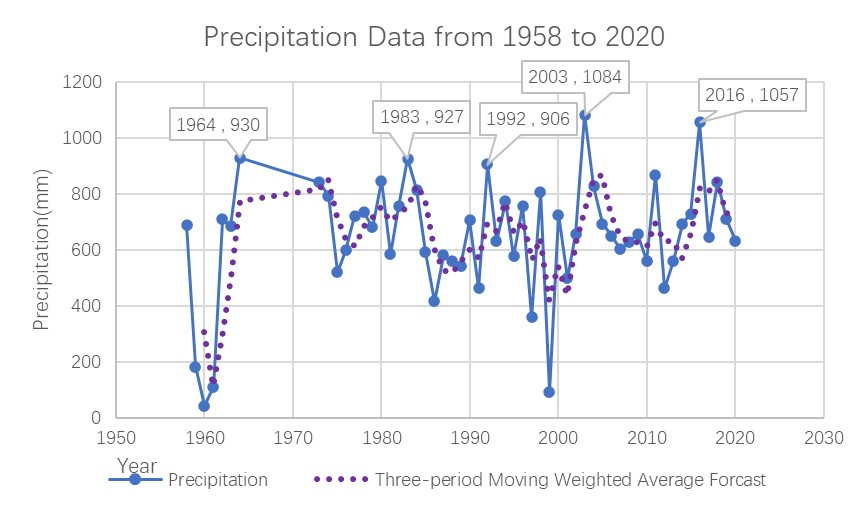
\includegraphics[width=0.8\textwidth]{precipitation_figure.jpg}
    \caption{Precipitation Data from 1958 to 2020}
    % \label{fig:label}
\end{figure}
\par
From 1958 to 2020, the annual average precipitation in Zhengzhou was 654 mm. Through the method of linear regression, the change trend line of precipitation can be obtained. At the same time, the regression coefficient can reflect the tendency rate of climate variables, that is, the average annual change of climate variables.
\par
Combined with the data set, it is easy to get the equation of trend line as follows:
\par
\begin{center}
    $ y = 2.6857x - 4696.4 $
\end{center}
\par
It can be seen that the annual average precipitation in Zhengzhou in recent 60 years has an upward trend. According to the above line chart, it can be found that the years with high precipitation are 1964, 1983, 1992, 2003 and 2016, with annual precipitation of 930mm, 927mm, 906mm, 1084mm and 1057mm respectively, all of which exceed 900mm.
\par
In addition, from the above line chart, it can be intuitively observed that the rainy periods are mainly around 1964, 1982~1984 and around 2002. The rainfall periods were mainly from 1965 to 1981 and from 1985 to 2001. At the same time, from the line chart, it can be directly observed that the precipitation in Zhengzhou has a certain periodicity, is constantly oscillating, and there is a sudden change at the same time. Through the method of three-period moving weighted average, the trend line of precipitation in Zhengzhou in recent 70 years can be made.
\par
\subsection{Quantitative Analysis of the
    Inundation Event of Zhengzhou in 2021}
\par
\hspace{1.25em}In the "July 20th" torrential rain in Zhengzhou in 2021, the precipitation in Zhengzhou has exceeded its annual average in just a few days. According to the data provided by the three observation stations, the heavy rainfall started on July 18th and lasted for about 4 days until July 22nd. Our team consulted the relevant data of China Meteorological Observatory Network, and learned that the strongest period of this heavy rainfall is from 19th to 20th, which is consistent with the data provided. On July 20th, 2021, the precipitation recorded by the three stations was 7.43 inches (about 189mm), 5.46 inches (about 139mm) and 3.22 inches (about 82mm), respectively. At the same time, from 16: 00 to 17: 00 on July 20th, Zhengzhou's maximum hourly rainfall reached 201.9mm, which broke through the historical extreme value of hourly rainfall in Chinese mainland. The 3-hour maximum rainfall in Zhengzhou reached 333mm. It can be seen that this heavy rainfall process has the characteristics of heavy rainfall, long time, short-term heavy rainfall and prominent precipitation extremes.
\par
By the afternoon of August 2nd, according to the news released by the Information Office of Henan Provincial People's Government, the flooding in Zhengzhou has caused 292 people to be killed and 47 people to be missing. There were 30,106 collapsed houses and 89,001 houses in the province, with 8.72 million mu of crops, 3.8 million mu of crops and 114.269 billion yuan of direct economic losses.
\par
\begin{figure}[h!t]
    \centering
    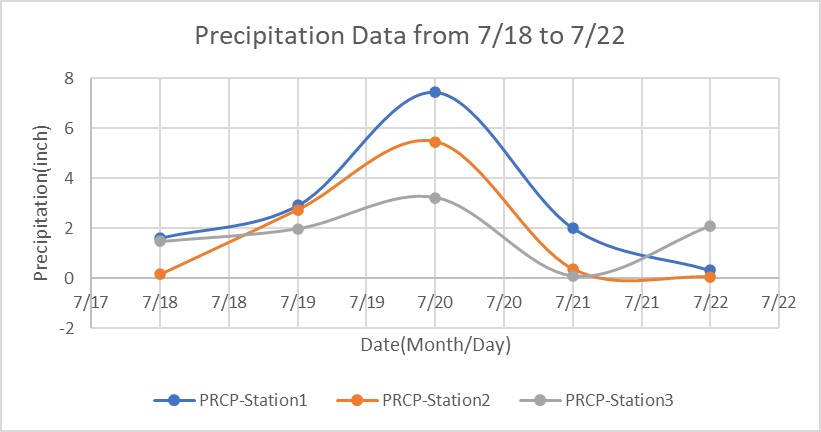
\includegraphics[width=0.8\textwidth]{precipitation_month_day.jpg}
    \caption{Precipitation Data from 7/18 to 7/22}
    % \label{fig:label}
\end{figure}


\section{Question 2. Analysis Precipitation Trend by ARIMA}

\subsection{Data Source}
\hspace{1em}
The data source of this model is the open meteorological data of the National Oceanic and Atmospheric Administration. By accessing the Global Surface Summary of the Day–GSOD database of this website, our team inquired and downloaded the meteorological data of five cities in Beijing, Guangzhou, Yinchuan, Dalian and Jinan from 1956 to 2021 for nearly 70 years. The meteorological indicators included in these meteorological data are consistent with those of three stations in Zhengzhou in Question 1.
\par
To analyze the trend of precipitation, the independent variable is time and the dependent variable is precipitation. By making the relationship images of precipitation in five cities with time, we can roughly analyze the precipitation trends in these five cities. At the same time, the ARIMA model has excellent performance in long-time series prediction, and it can also complete the analysis of precipitation trend.

\subsection{Model Analysis and Symbols}
\hspace{1em}
The most important point of constructing ARIMA model lies in the stationarity of time series data. Stationarity means that the fitting curve obtained from the sample time series can continue inertially along the existing shape in a short time in the future, that is, the mean and variance of the data should not change too much in theory. Therefore, the first step is to observe whether the data is a stationary time series. For the non-stationary time series, the D-order difference operation should be carried out first, and it should be transformed into a stationary time series.
\par
After obtaining the stationary time series, the autocorrelation coefficient ACF and partial autocorrelation coefficient PACF should be calculated for the stationary time series respectively. By analyzing the autocorrelation diagram and partial autocorrelation diagram, we can get the parameters $p$ and $q$, and finally build the following ARIMA model:
\begin{center}
    $\hat{y_t} = \mu + \phi_1*y_{t-1} + ... + \phi_{p}*y_{t-p} + \theta_1*e_{t-1} + ... + \theta_q*e_{t-1} $
\end{center}
\par
In this paper, we use symbol $ARIMA_{city}(p,d,q)$ to describe the ARIMA model of each city.

\subsection{Model Building}
\hspace{1.25em}(1)Test the stationarity of the given time series:
\par
In this paper, we use ADF test is to judge whether the time series is stationary or not. ADF test results are as follows:
\par
\begin{center}
    \begin{table}[h!t]
        \caption{ADF Test Results}
        \begin{tabular}{lccccc}
        \hline
                                    & Beijing    & Guangzhou  & Jinan      & Dalian     & Yinchuan   \\ \hline
        Diff(parameter $d$)                       & 2          & 2          & 1          & 2          & 1          \\
        Test Statistic Value        & -11.30647  & -4.0139922 & -8.891108  & -5.7975579 & -9.0399174 \\
        p-value                     & 1.27E-20   & 1.34E-03   & 1.24E-14   & 4.71E-07   & 5.17E-15   \\
        Lags Used                   & 0          & 5          & 1          & 3          & 1          \\
        Number of Observations Used & 53         & 47         & 52         & 49         & 51         \\
        Critical Value(1\%)         & -3.5602424 & -3.577848  & -3.5628785 & -3.5714715 & -3.5656241 \\
        Critical Value(5\%)         & -2.9178502 & -2.9253381 & -2.9189733 & -2.9226295 & -2.9201422 \\
        Critical Value(10\%)        & -2.5967964 & -2.6007735 & -2.5973934 & -2.5993358 & -2.5980147 \\ \hline
        \end{tabular}
        \end{table}
\end{center}
\par
Because the ADF test values are all less than -3.56024, and noting that the p-values in all ADF test results are very small, we can reject the original non-stationary hypothesis and think that these time series are stable.
\par
(2)Obtain parameters $p$ and $q$
\par
In order to determine parameters $p$ and $q$, ACF diagram (autocorrelation diagram) and PACF diagram (partial autocorrelation diagram) need to be made. Where p is the order of autoregressive model and q is the order of moving average model. Parameter $p$ can be determined by ACF diagram and parameter $q$ can be determined by PACF diagram.
\par
The following figure is ACF chart and PACF chart of Beijing precipitation series data:
\begin{figure}[h!t]
    \centering
    \subfigure[ACF Figure]{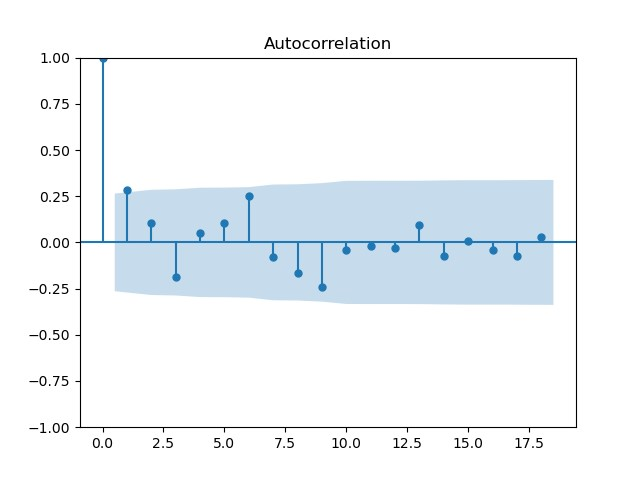
\includegraphics[width=0.485\linewidth]{beijing_acf.jpg}}\hfill
    \subfigure[PACF Figure]{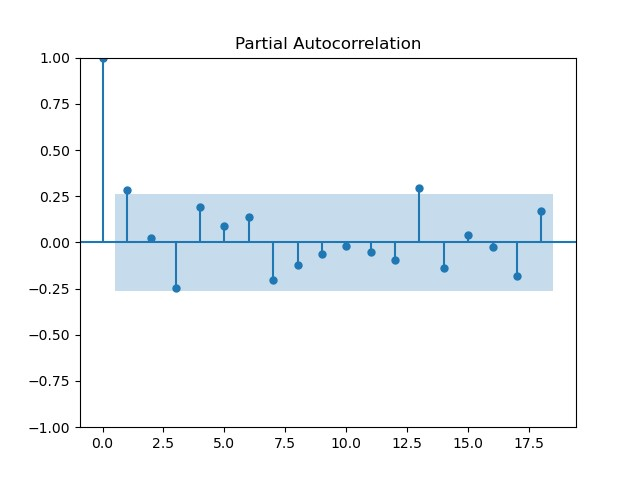
\includegraphics[width=0.485\linewidth]{beijing_pacf.jpg}}
\end{figure}
\par 
Therefore, it can be determined that for Beijing precipitation series data, the parameter $p$ in ARIMA model should be 0 and the parameter $q$ should be 1.
\par
The following figure is ACF chart and PACF chart of Guangzhou precipitation series data:
\begin{figure}[h!t]
    \centering
    \subfigure{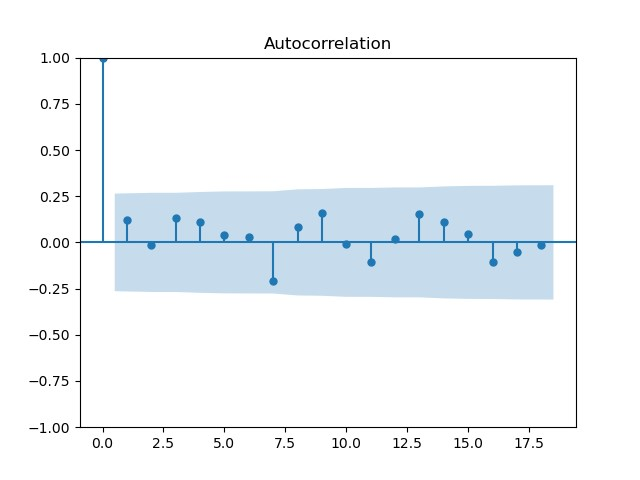
\includegraphics[width=0.485\linewidth]{guangzhou_acf.jpg}}\hfill
    \subfigure{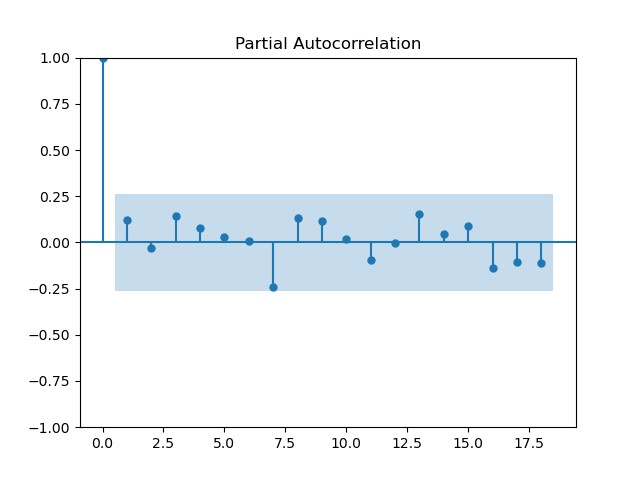
\includegraphics[width=0.485\linewidth]{guangzhou_pacf.jpg}}
\end{figure}
\par 
Similarly, the parameter $p$ in ARIMA model should be 1 and the parameter $q$ should be 1.
\par
The following figure is ACF chart and PACF chart of Yinchuan precipitation series data:
\begin{figure}[h!t]
    \centering
    \subfigure{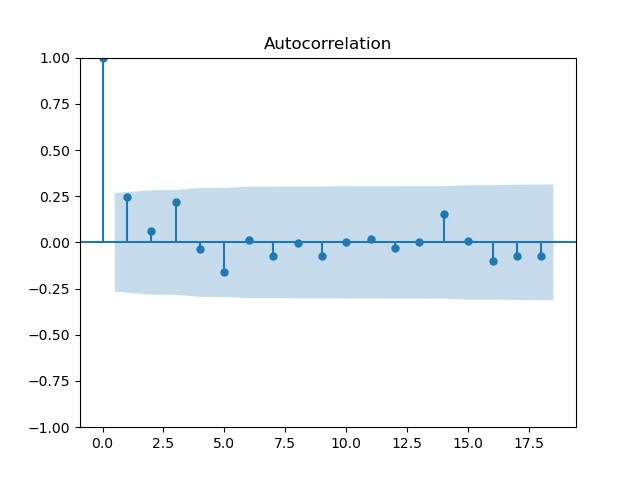
\includegraphics[width=0.485\linewidth]{yinchuan_acf.jpg}}\hfill
    \subfigure{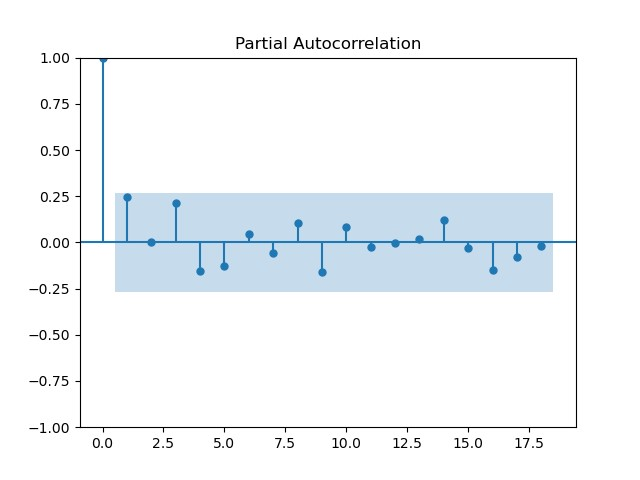
\includegraphics[width=0.485\linewidth]{yinchuan_pacf.jpg}}
\end{figure}
\par 
The parameter $p$ in ARIMA model should be 1 and the parameter $q$ should be 1.
\newpage
\par
The following figure is ACF chart and PACF chart of Jinan precipitation series data:
\begin{figure}[h!t]
    \centering
    \subfigure{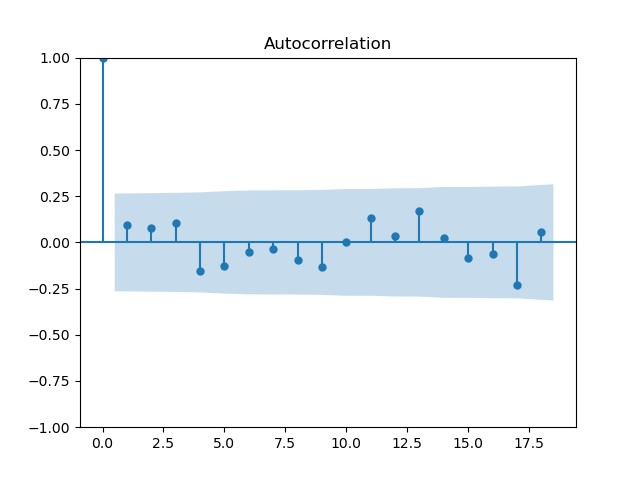
\includegraphics[width=0.485\linewidth]{jinan_acf.jpg}}\hfill
    \subfigure{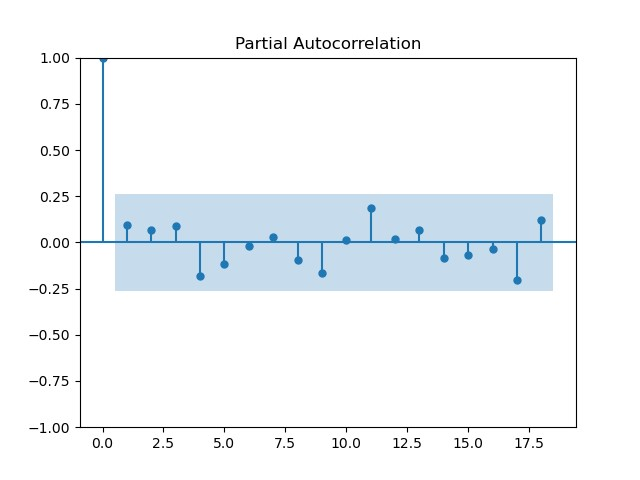
\includegraphics[width=0.485\linewidth]{jinan_pacf.jpg}}
\end{figure}
\par 
The parameter $p$ in ARIMA model should be 2 and the parameter $q$ should be 0.
\par
The following figure is ACF chart and PACF chart of Dalian precipitation series data:
\begin{figure}[h!t]
    \centering
    \subfigure{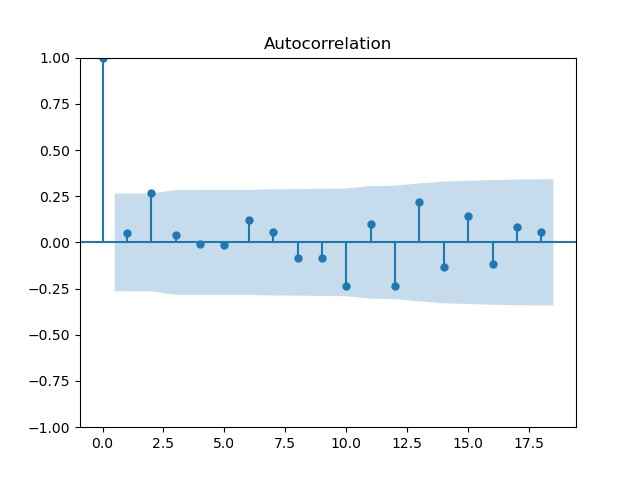
\includegraphics[width=0.485\linewidth]{dalian_acf.jpg}}\hfill
    \subfigure{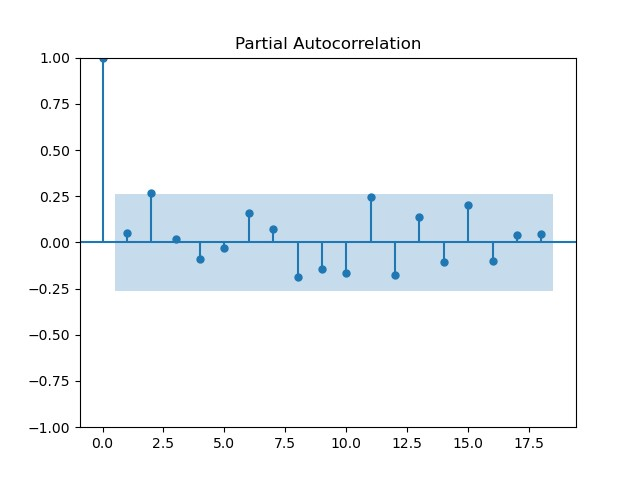
\includegraphics[width=0.485\linewidth]{dalian_pacf.jpg}}
\end{figure}
\par 
The parameter $p$ in ARIMA model should be 1 and the parameter $q$ should be 1.
\par
According to the previously obtained parameters, five ARIMA models can be constructed:
\par
\begin{center}
    \par
    $ARIMA_{Beijing}(0,1,1)$
    \par 
    $ARIMA_{Guangzhou}(1,2,1)$
    \par 
    $ARIMA_{Dalian}(1,2,1)$
    \par 
    $ARIMA_{Jinan}(2,1,0)$
    \par 
    $ARIMA_{Yinchuan}(1,1,1)$
\end{center}
\par 
After building ARIMA model, the precipitation change maps of five cities can be made separately. From the figure, we can directly observe the change trend of precipitation. The blue line is the true value and the purple line is the predicted value of ARIMA model. It can be seen from the figure that the model fits well.
\begin{figure}[h!t]
    \centering
    \subfigure[Beijing]{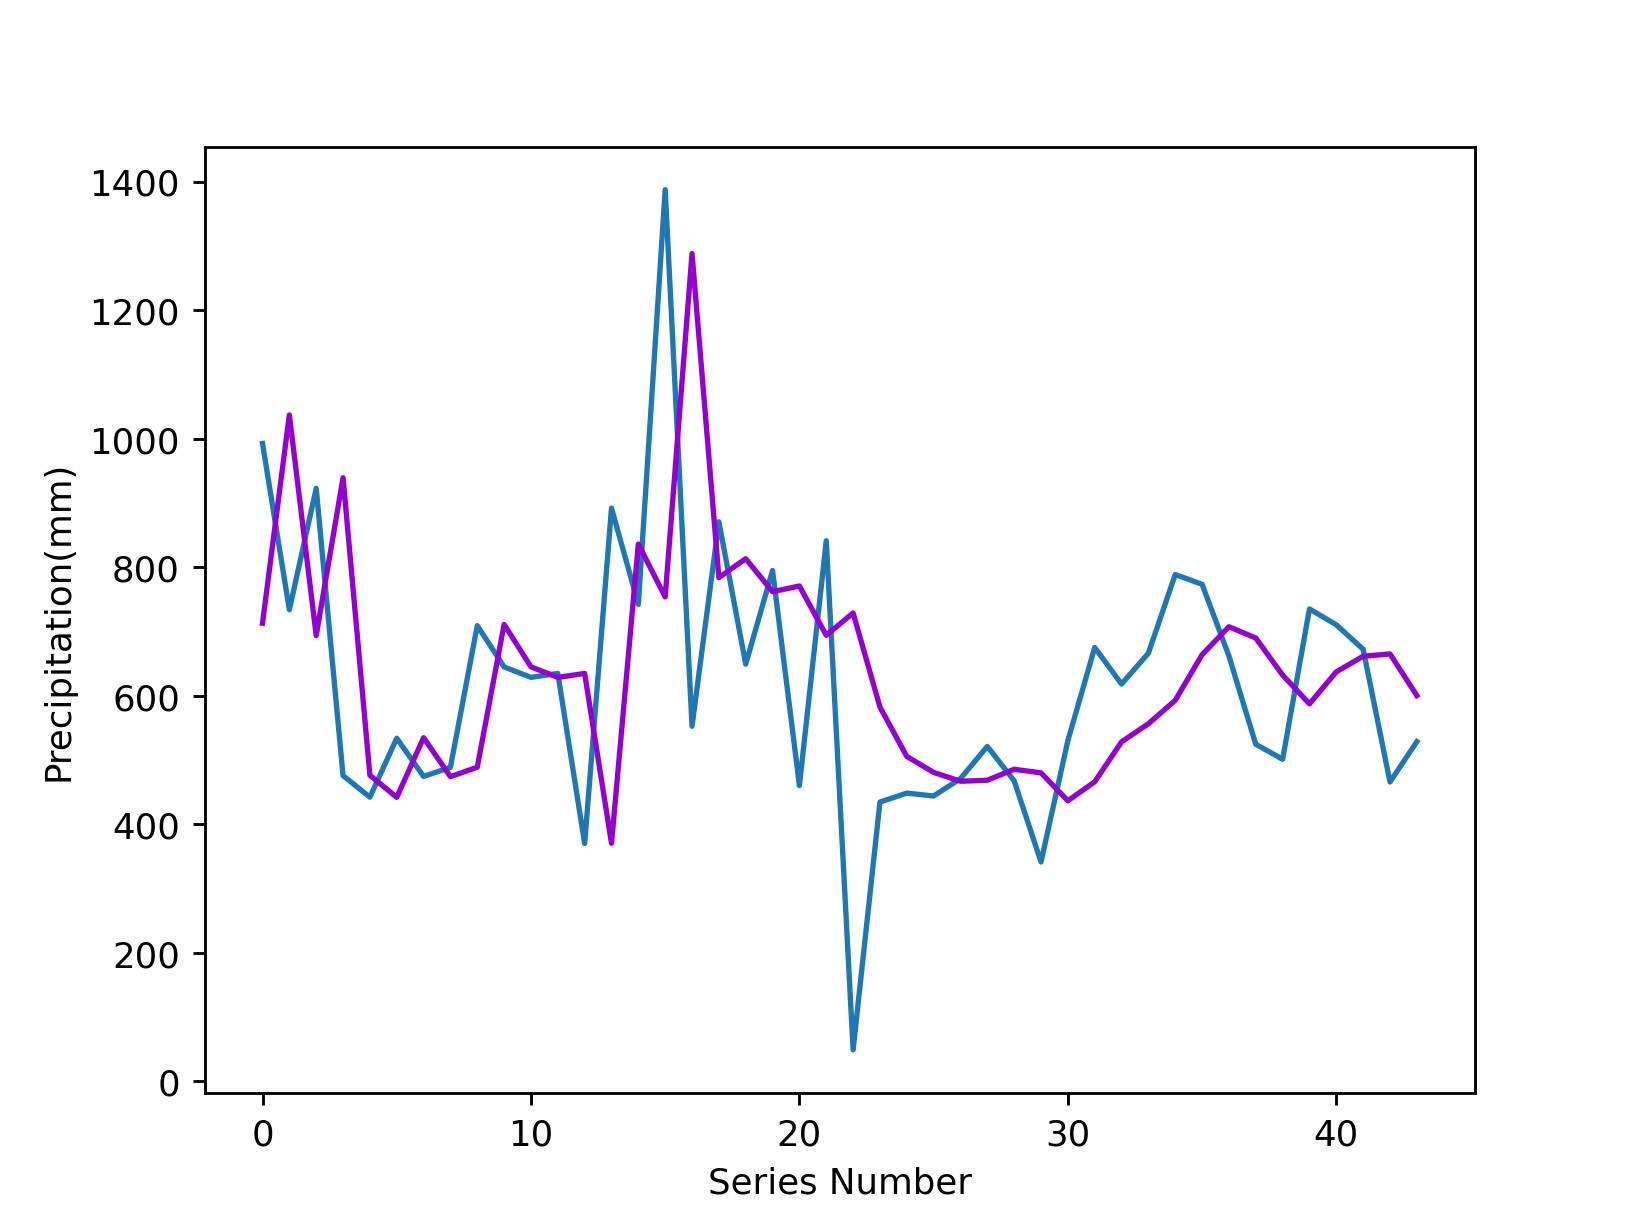
\includegraphics[width=0.485\linewidth]{beijing_arima.jpg}}\hfill
    \subfigure[Beijing]{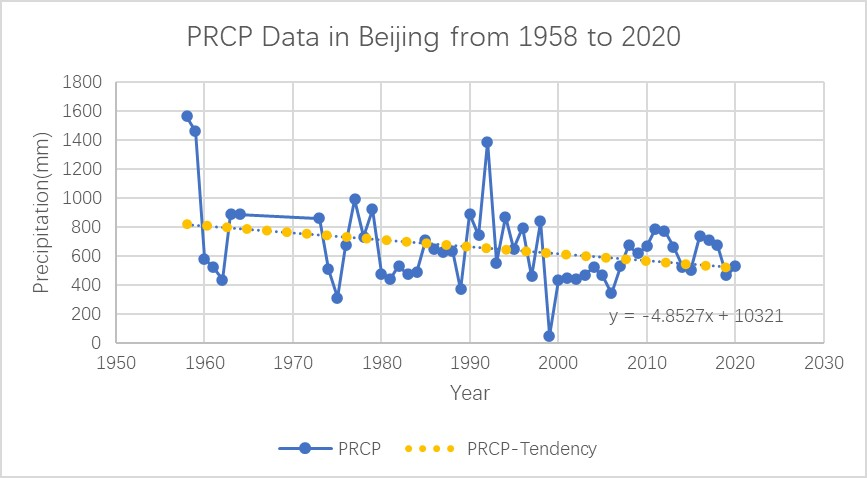
\includegraphics[width=0.485\linewidth]{prcp_beijing.jpg}}
\end{figure}
\begin{figure}[h!t]
    \centering
    \subfigure[Guangzhou]{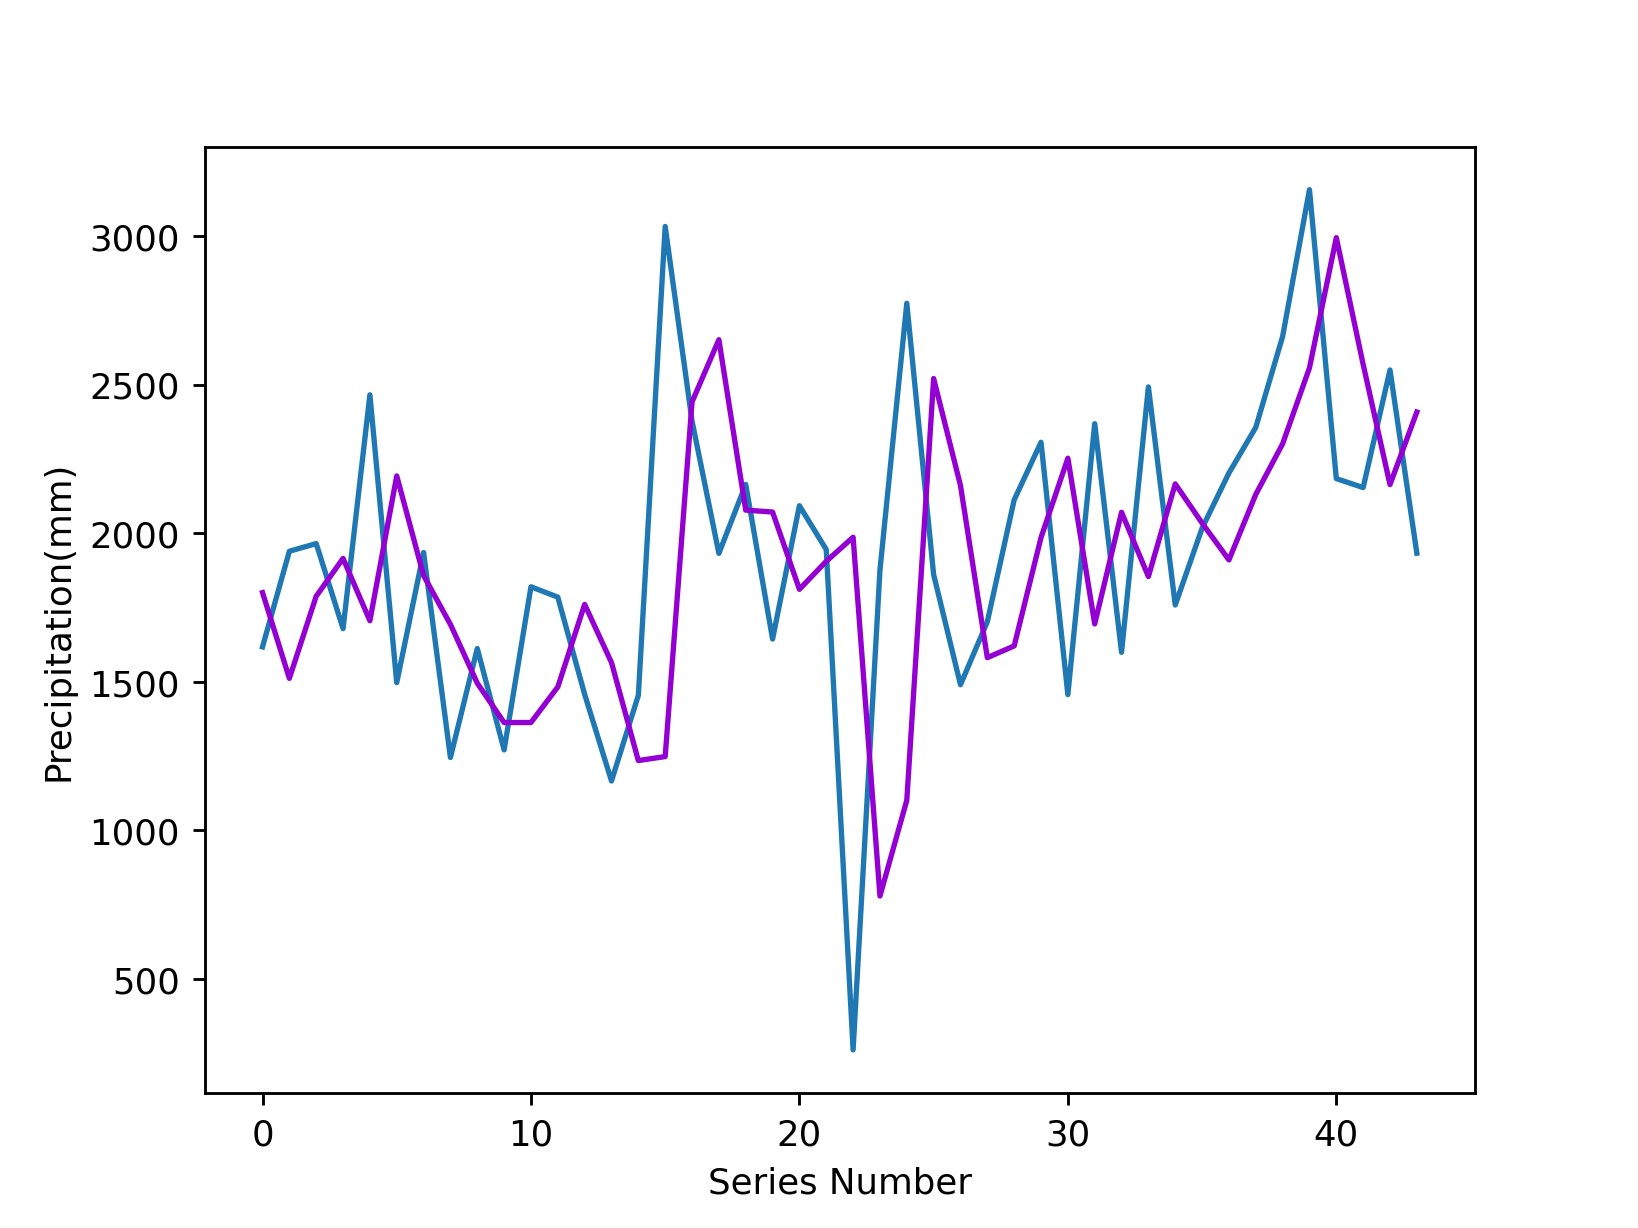
\includegraphics[width=0.485\linewidth]{guangzhou_arima.jpg}}\hfill
    \subfigure[Guangzhou]{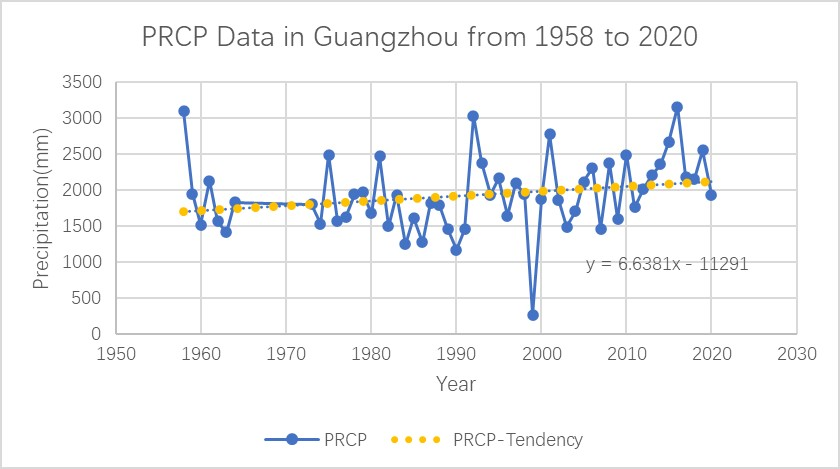
\includegraphics[width=0.485\linewidth]{prcp_guangzhou.jpg}}
\end{figure}
\begin{figure}[h!t]
    \centering
    \subfigure[Dalian]{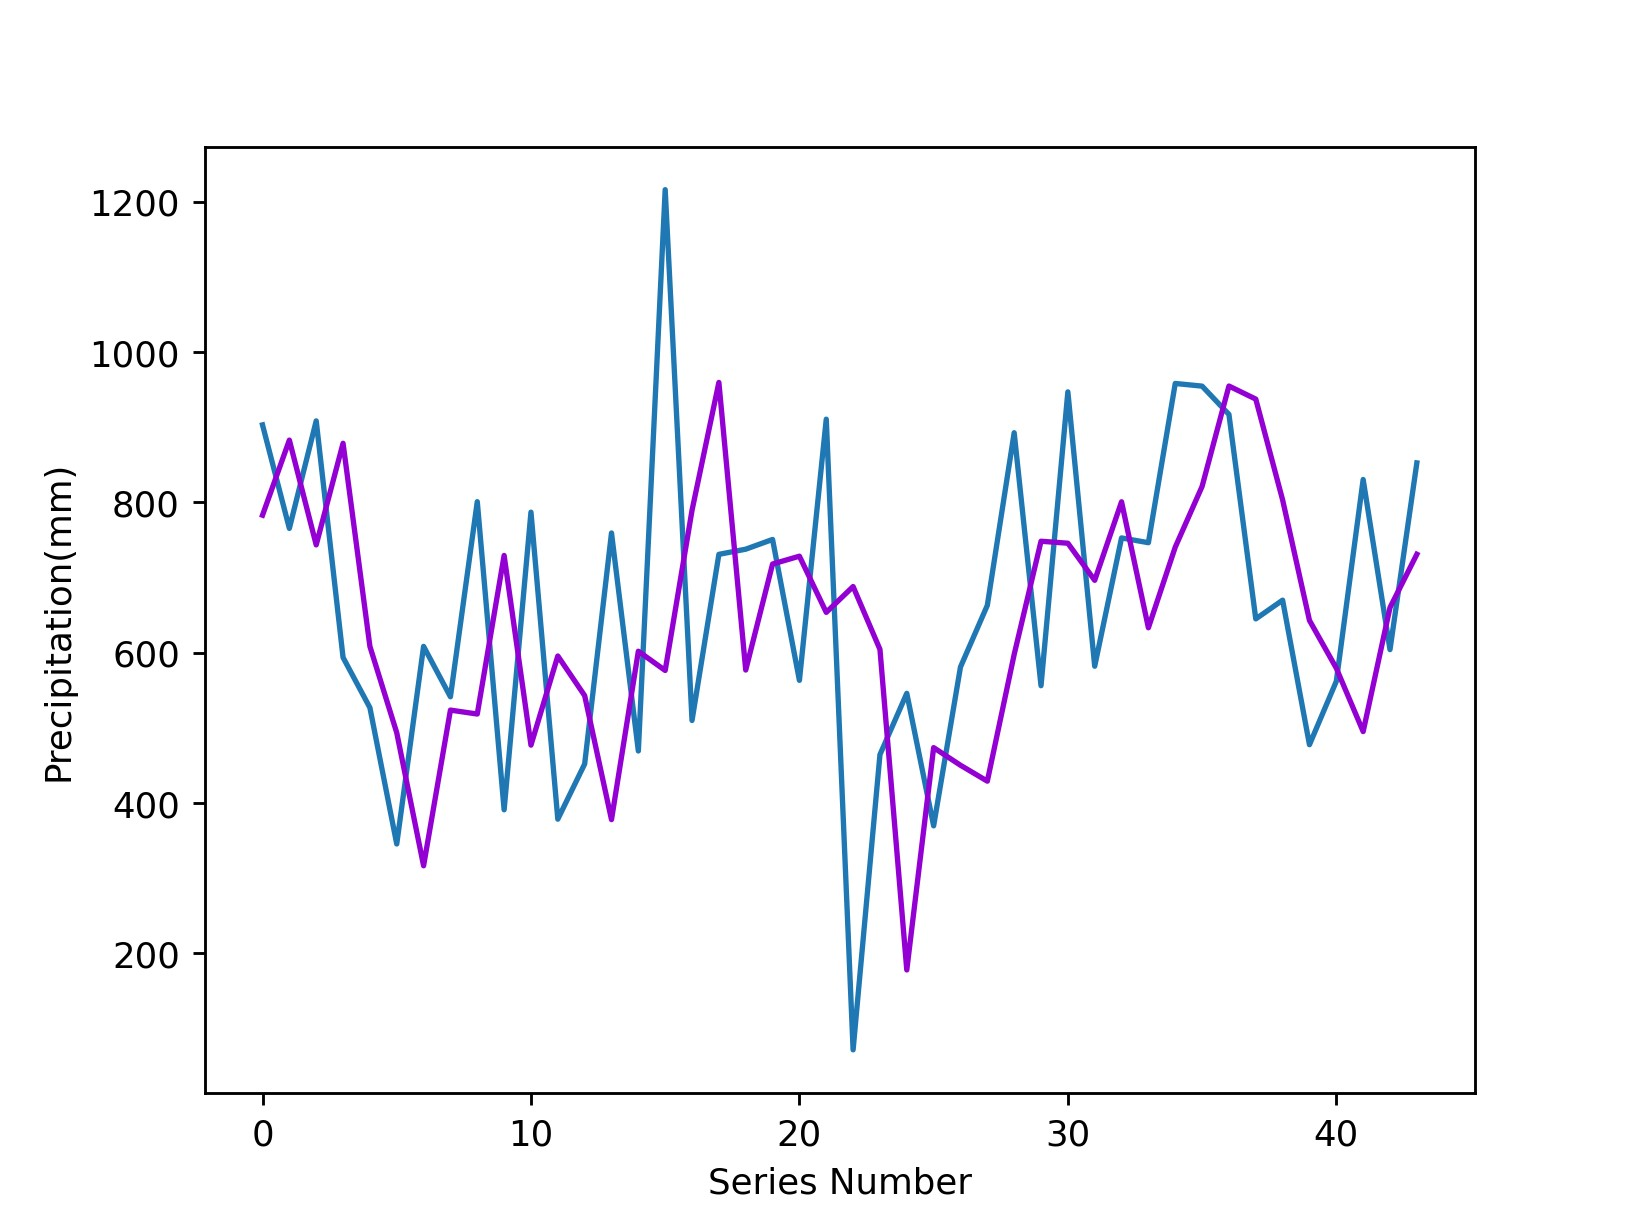
\includegraphics[width=0.485\linewidth]{dalian_arima.jpg}}\hfill
    \subfigure[Dalian]{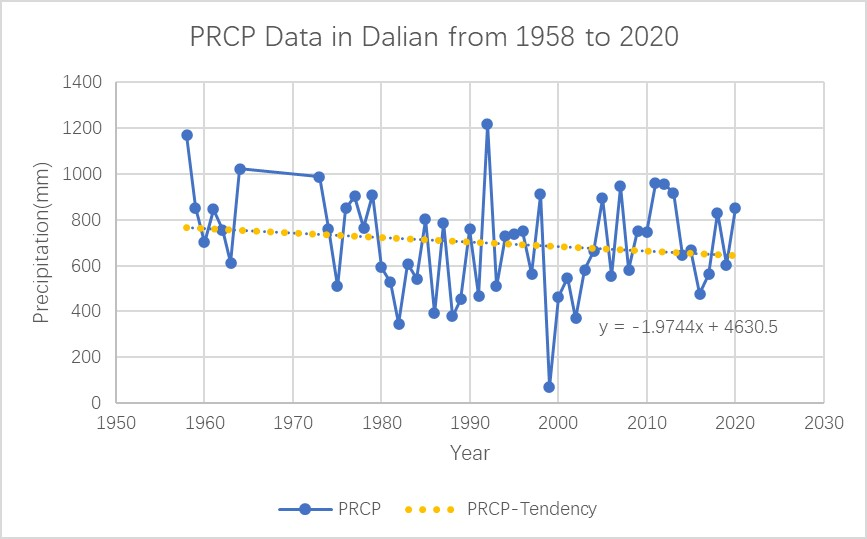
\includegraphics[width=0.485\linewidth]{prcp_dalian.jpg}}
\end{figure}
\begin{figure}[h!t]
    \centering
    \subfigure[Jinan]{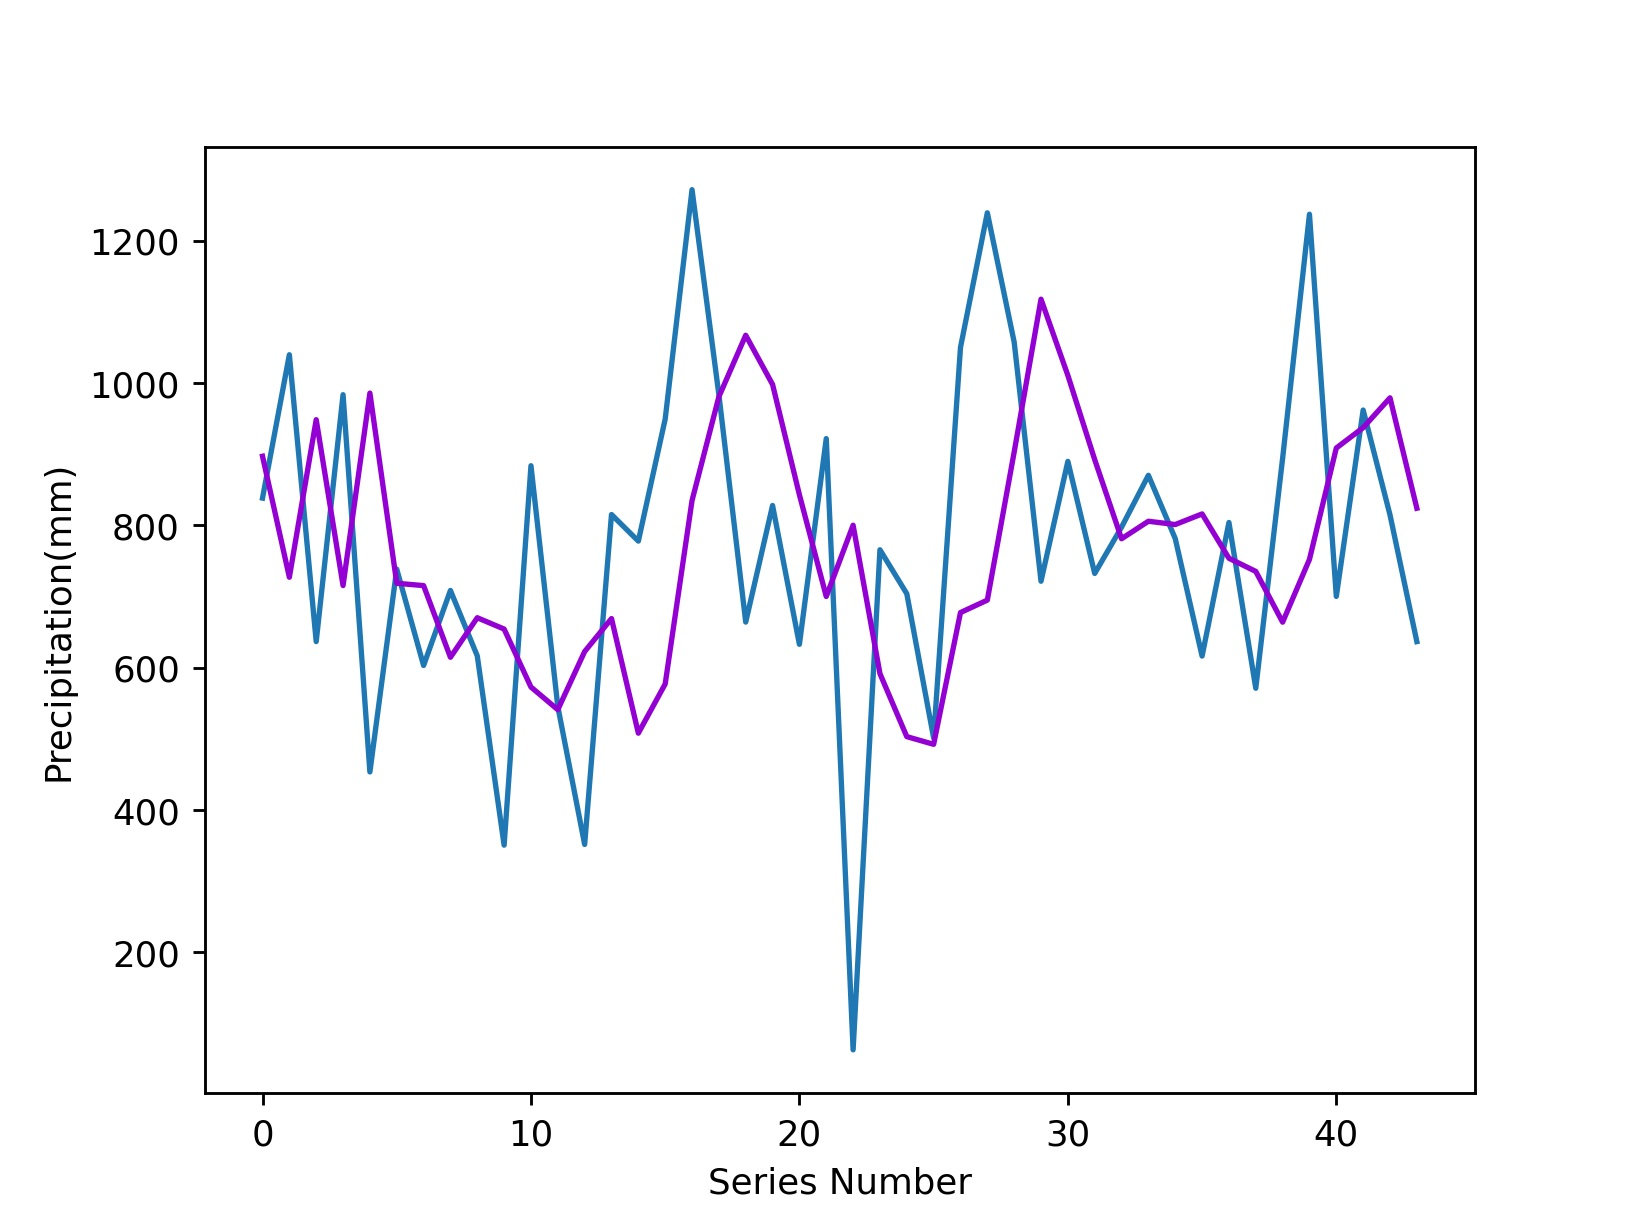
\includegraphics[width=0.485\linewidth]{jinan_arima.jpg}}\hfill
    \subfigure[Jinan]{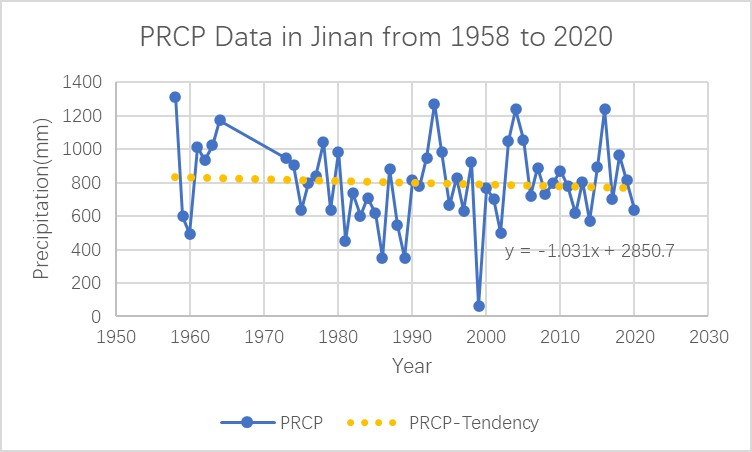
\includegraphics[width=0.485\linewidth]{prcp_jinan.jpg}}
\end{figure}
\begin{figure}[h!t]
    \centering
    \subfigure[Yinchuan]{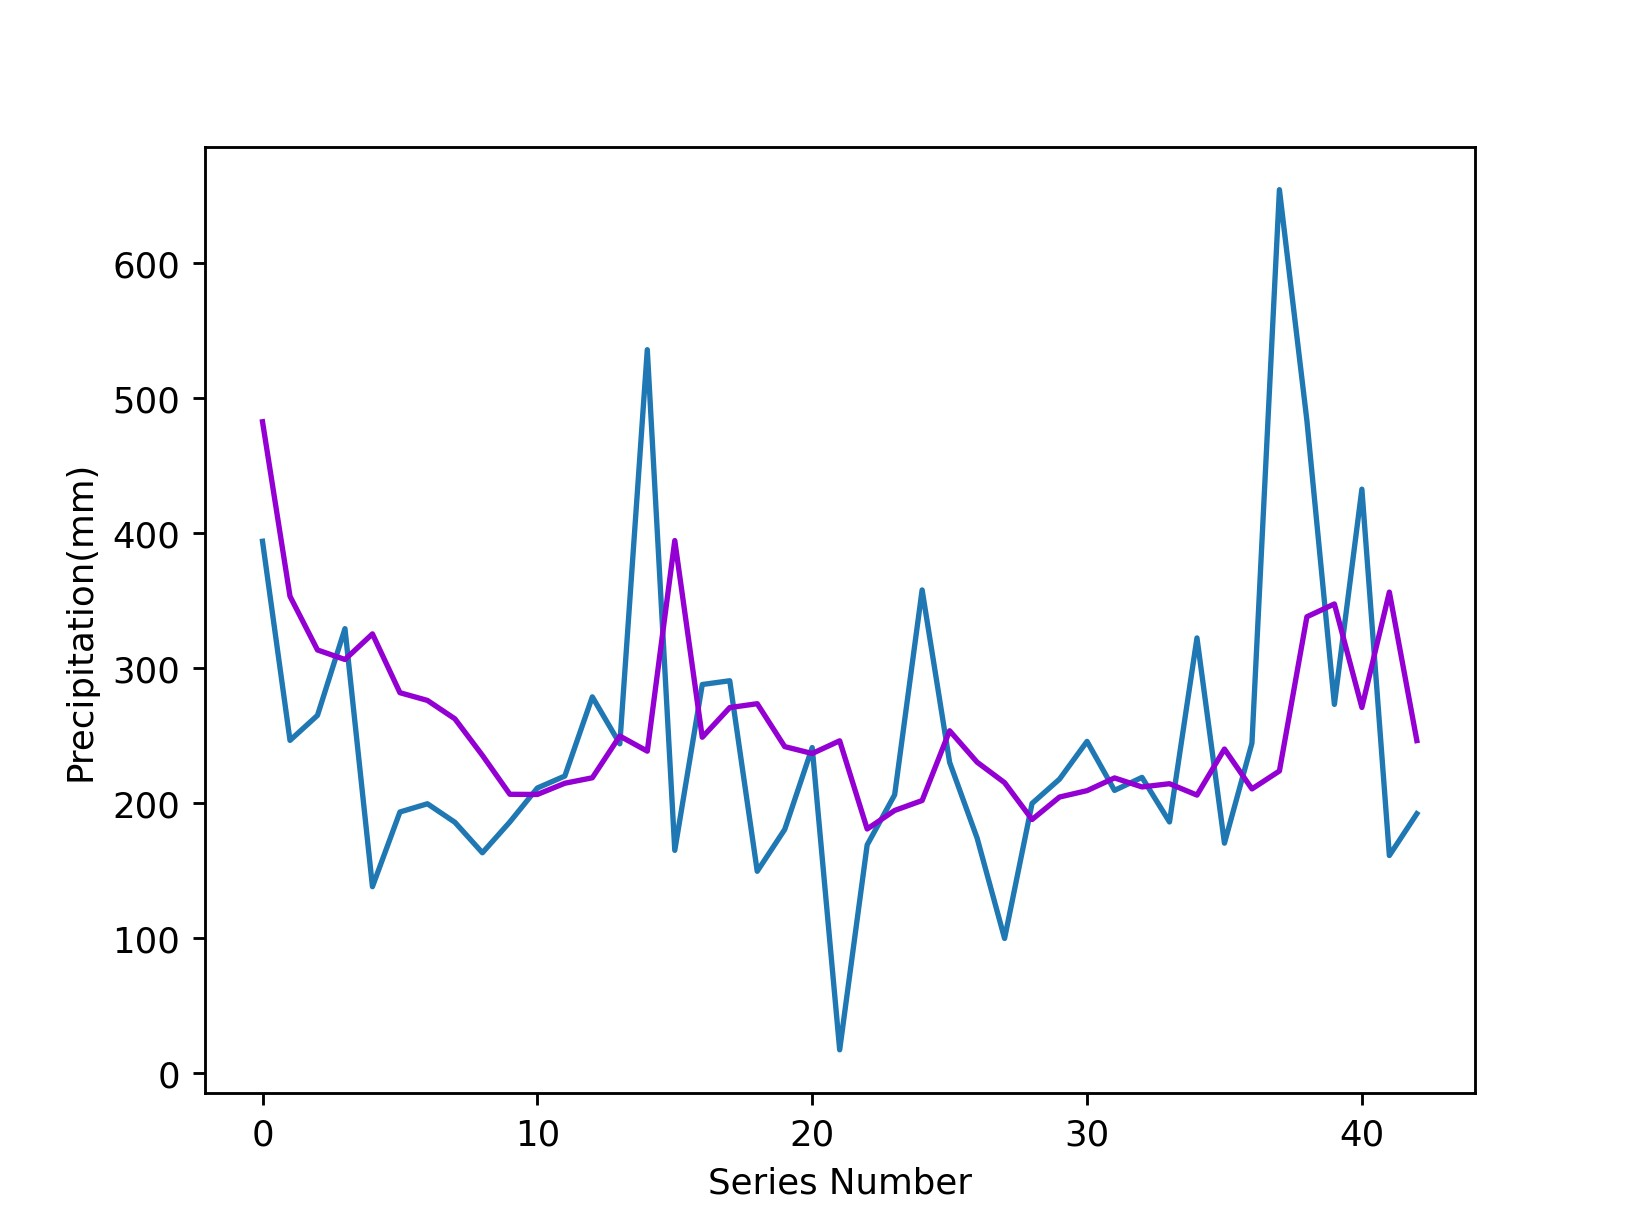
\includegraphics[width=0.485\linewidth]{yinchuan_arima.jpg}}\hfill
    \subfigure[Yinchuan]{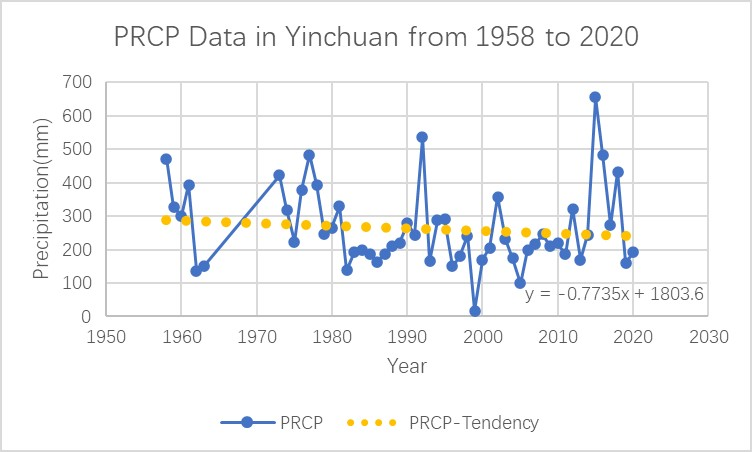
\includegraphics[width=0.485\linewidth]{prcp_yinchuan.jpg}}
\end{figure}


\subsection{Precipitation Trend Analysis}
\subsubsection{Beijing}
\hspace{1.25em}From 1958 to 2020, the annual average precipitation in Beijing was 654 mm. According to the chart made before, it can be found that the years with higher precipitation are 1958, 1959 and 1992, with an interval of about 30 years. The annual precipitation is 1566mm, 1463mm and 1388mm respectively, all exceeding 1300 mm.
\par 
Besides, the rainy periods in Beijing are mainly from 1958 to 1959 and 1992. The periods of low rainfall were mainly from 1960 to 1991 and from 1992 to 2020. It can be found that the precipitation in Beijing has a cycle of 15 years on average, which is very periodic. At the same time, the precipitation is concentrated in 400mm~1000mm, and has a decreasing trend. According to the trend line, the annual precipitation in Beijing decreases by about 48mm every 10 years on average.
\subsubsection{Dalian}
\hspace{1.25em}
From 1958 to 2020, the annual average precipitation in Dalian was 697 mm. It can be found that the years with higher precipitation are 1964, 1973, 1992, 2007 and 2011-2013, with intervals of about 4 years or 10-20 years. The annual precipitation is 1023mm, 988mm, 1216mm, 947mm, 958mm, 955mm and 917mm respectively, all of which exceed 900mm.
\par 
Besides, the rainy periods in Dalian are mainly in 1958, 1964, 1973, 1992, 2007 and 2011-2013. The main periods of low rainfall were 1963, 1975, 1980~1984, 1988~1989 and 1999~2003. At the same time, the annual precipitation in Dalian is concentrated in 400 ~ 1000 mm. According to the trend line, the annual precipitation in Dalian decreases by about 20mm every 10 years on average.
\subsubsection{Guangzhou}
\hspace{1.25em}
From 1958 to 2020, the annual average precipitation in Guangzhou was 1932 mm. It can be found that the years with higher precipitation are 1958, 1975, 1981, 1992, 2001 and 2016, with an interval of about 6~16 years. The annual precipitation is 3095mm, 2488mm, 2466mm, 3032mm, 2774mm and 3156mm respectively, all exceeding 2450mm.
\par
Besides, the rainy periods in Guangzhou are mainly from 1958 to 1959, 1992, 2001 and 2013 to 2016. The main periods of low rainfall were 1962~1963, 1976~1977, 1984~1991, 1996~2000 and 2002~2004. At the same time, the annual precipitation in Guangzhou is concentrated in 1000~2500mm, with an upward trend, without obvious periodicity. According to the trend line, the average annual precipitation in Guangzhou increases by about 66mm every 10 years.
\subsubsection{Jinan}
\hspace{1.25em}
From 1958 to 2020, the annual average precipitation in Jinan was 797 mm. The annual average precipitation of Jinan in recent 60 years has a slight downward trend. It can be found that the years with higher precipitation are 1958, 1961, 1963-1964, 1978, 1993, 2003-2005 and 2016, with intervals of about 3 or 15 years. The annual precipitation is 1312mm, 1014mm, 1024mm, 1172mm, 1040mm, 1271mm, 1050mm, 1239mm, 1057mm and 1237mm respectively, all of which exceed 1000mm.
\par 
Besides, the rainy periods in Jinan are mainly from 1961 to 1974, 1992 to 1994, 2001 and 2015 to 2019. The rainfall periods were mainly from 1959 to 1960, from 1981 to 1991 and from 1995 to 2002. At the same time, the annual precipitation in Jinan is concentrated in 500 ~ 1000 mm. According to the trend line, the average annual precipitation in Jinan decreases by about 10mm every 10 years, which is not obvious.
\subsubsection{Yinchuan}
\hspace{1.25em}
From 1958 to 2020, the annual average precipitation in Yinchuan was 262 mm. The annual average precipitation in Yinchuan in recent 60 years has a slight downward trend. The years with high precipitation are 1958, 1973, 1977, 1992, 2015-2016 and 2018, with intervals of about 5 or 15 years.
\par 
Besides, the rainy periods in Yinchuan are mainly from 1958 to 1961, from 1973 to 1978, around 1992 and from 2015 to 2018. The rainfall periods were mainly from 1962 to 1963, from 1982 to 1991 and from 1993 to 2013. As an inland city, Yinchuan's precipitation shows a certain periodicity, with an average cycle of about every 10 years. According to the trend line, the annual average precipitation in Yinchuan decreases by about 7mm every 10 years.
\section{Question 3. Use LSTM TO Predict and Analyze Potential Cities with Extreme Rainfall}
\subsection{Data Source}
\hspace{1.25em}
The data of this model comes from the records from January 1st, 2020 to November 9th, 2021 provided by Beijing Meteorological Observatory. These records contain indicators such as dewp max min MX SPD prcp temp visib wdsp, which have the same meaning as those defined in model 1.

\subsection{Model Analysis and Symbols}
\hspace{1.25em}
Long-term and short-term memory cyclic neural network is a special form derived from RNN model. Its purpose is to solve the problems of gradient disappearance and gradient explosion in cyclic neural network. It can better preserve long-term memory by updating the gate structure and cell state, and solve the problems of gradient disappearance and gradient explosion by retaining time-related information in the storage unit.
\par
The chain structure inside the hidden layer of LSTM neural network is shown in the figure below:
\begin{figure}[h!t]
    \centering
    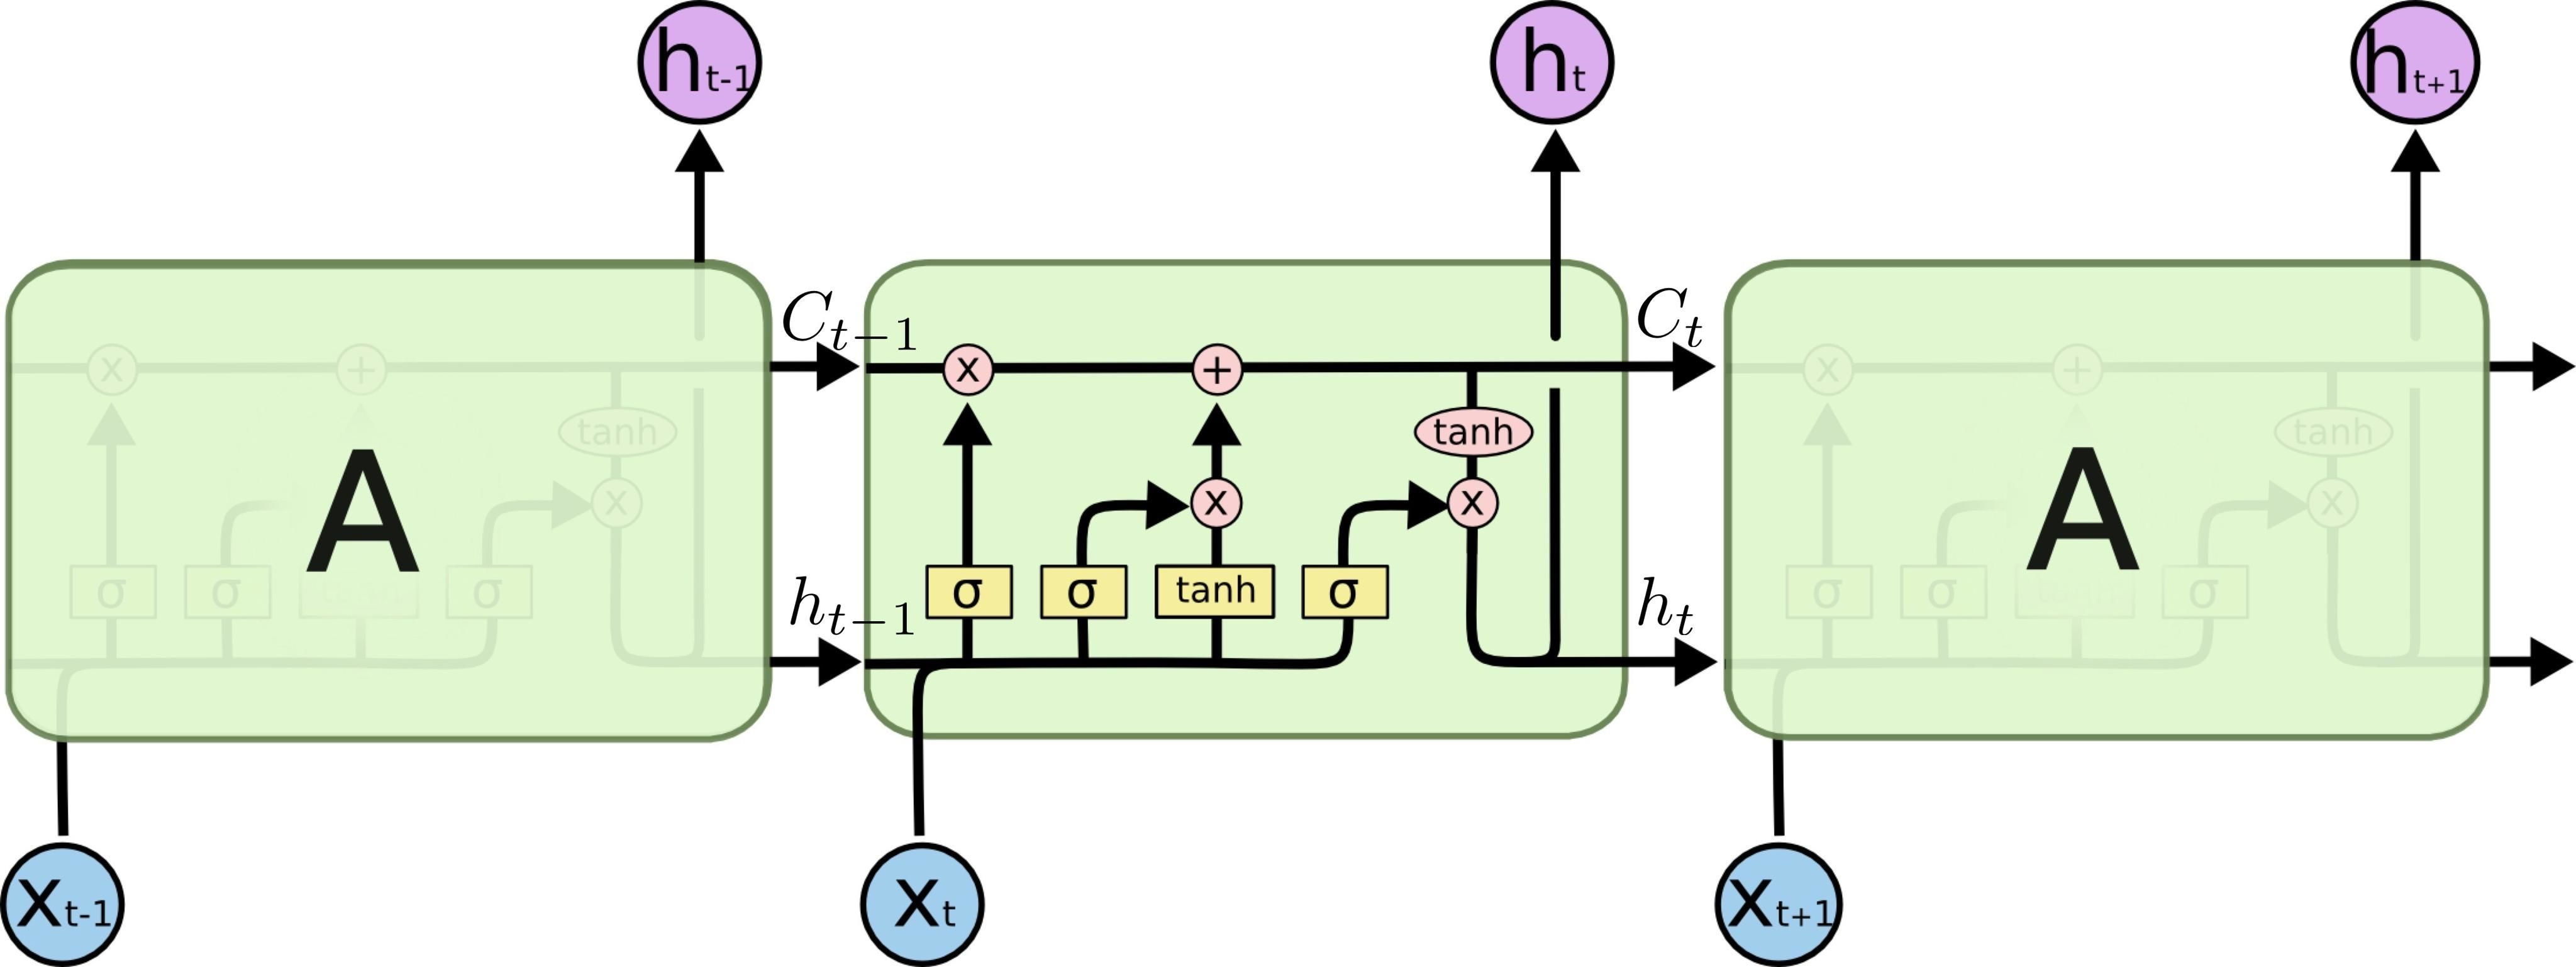
\includegraphics[width=0.8\textwidth]{LSTM_unit.jpg}
    \caption{LSTM unit}
    % \label{fig:label}
\end{figure}
\par 
The internal structure of each Memory Cell has three gate structures, namely, forget gate, input gate and output gate.

\subsection{Model Building}
\hspace{1.25em}
(1)The first step in LSTM is to decide what information we will discard from the cell state. This decision is made through a layer called Forgetting Door. The gate will read $h_{t-1}$ and $x_{t}$, and output a value between 0 and 1 to each number in cell state $C_{t-1}$. 1 means "completely reserved" and 0 means "completely abandoned".
\par
(2)The next step is to determine what new information is stored in the cell state. There are two parts here. First, the $sigmoid$ layer is called the "input gate layer", which determines what value we will update. Then, a $tanh$ layer creates a new candidate vector, $\tilde{C_{t}} $, which will be added to the state. Next, we will talk about these two information to generate the update of the status.
\par
(3)Then it is to update the state of the old cells. $C_{t-1}$ is updated to $C_{t}$. The previous steps have already decided what will be done, and now we are actually doing it.
\par 
We can multiply the old state by $f_{t}$, and discard the information that we determine to be discarded, then add $i_t*\tilde{C_{t}}$. This is the new candidate value, which changes according to the degree to which we decide to update each state.
\par
(4)potential cities with extreme rainfall. We can collect meteorological information from several cities and predict the date of high probability precipitation by LSTM model.

\section{Strengths and Weakness}
\hspace{1.5em}
The strengths of this paper is the visualization of a large amount of data, which makes the article illustrated.
\par
At the same time, the data is well preprocessed, and the meteorological documents can be consulted to analyze the causes of abnormal values, thus avoiding data problems in the modeling process.
\par
The weakness of this paper is that due to the limitation of the team's ability, all five questions could not be completed. At the same time, the specific modeling details are not elaborated too much in the text, but left in the code part. In the concrete modeling process, the verification of the model pays more attention to the image, but seldom adopts the quantitative method.

\section{References cite}
\hspace{1.25em}
National Oceanic and Atmospheric Administration at Ref.\cite{bib:one}
\par 
LSTM Model Analysis at Ref.\cite{bib:two}



%----------------------------参考文献

\begin{thebibliography}{9}%宽度9
    \bibitem{bib:one} \url{https://www.ncei.noaa.gov/access/search/index}
    \bibitem{bib:two} \url{https://www.jianshu.com/p/9dc9f41f0b29}

    \bibitem{bib4} Hochreiter, S, and J. Schmidhuber. “Long short-term memory.” Neural Computation 9.8(1997):1735-1780.

    \bibitem{bib5} Sussillo, D. (2014). Random walks: Training very deep nonlinear feed-forward networks with smart initialization.CoRR,abs/1412.6558. 248, 259, 260, 344

    \bibitem{bib6} Gers F A, Schmidhuber J, Cummins F. Learning to forget: Continual prediction with LSTM[J]. 1999.

    \bibitem{bib7} Yujia Jin and Caiwei Xiong and Jun Cao. Weather Conditions Prediction with Climate Change Dataset with Linear Regression Model, Autoregressive Model, LSTM Model[J]. International Core Journal of Engineering, 2021, 7(1)
\end{thebibliography}

% ---------------------开始附录

\newpage

\section*{Appendix}
% 在目录中添加Appendix
\addcontentsline{toc}{section}{Appendix}

\begin{lstlisting}[language=Python,caption={The Python Source code of PCA}]
    data = pd.read_excel(r'.\data\data.xlsx', index_col=0)
    sc = StandardScaler()
    data_std = sc.fit_transform(data)
    pca = PCA(n_components=4)
    pca.fit_transform(data_std)

\end{lstlisting}
\begin{lstlisting}[language=Python,caption={The Python Source code of ARIMA}]
    beijing_data = pd.read_excel(r'.\data\processed_beijing.xlsx', index_col=0, skiprows=0)
    dalian_data = pd.read_excel(r'.\data\processed_dalian.xlsx', index_col=0, skiprows=0)
    guangzhou_data = pd.read_excel(r'.\data\processed_guangzhou.xlsx', index_col=0, skiprows=0)
    jinan_data = pd.read_excel(r'.\data\processed_jinan.xlsx', index_col=0, skiprows=0)
    yinchuan_data = pd.read_excel(r'.\data\processed_yinchuan.xlsx', index_col=0, skiprows=0)
    
    beijing_prcp = beijing_data.get('PRCP')
    dalian_prcp = dalian_data.get('PRCP')
    guangzhou_prcp = guangzhou_data.get('PRCP')
    jinan_prcp = jinan_data.get('PRCP')
    yinchuan_prcp = yinchuan_data.get('PRCP')
    
    
    def adf_check(prcp):
        t = adfuller(prcp)  # ADF test
        output = pd.DataFrame(
            index=['Test Statistic Value', "p-value", "Lags Used", "Number of Observations Used", "Critical Value(1%)",
                   "Critical Value(5%)", "Critical Value(10%)"], columns=['value'])
        output['value']['Test Statistic Value'] = t[0]
        output['value']['p-value'] = t[1]
        output['value']['Lags Used'] = t[2]
        output['value']['Number of Observations Used'] = t[3]
        output['value']['Critical Value(1%)'] = t[4]['1%']
        output['value']['Critical Value(5%)'] = t[4]['5%']
        output['value']['Critical Value(10%)'] = t[4]['10%']
        return output
        # if ADF test value < {1%}, then stable
    
    
    def plot_acf_pacf(prcp):
        plot_acf(prcp)
        plot_pacf(prcp, method='ywm')
        plt.show()
    
    
    def auto_arima_model(data):
        train_size = 45
        test_size = data.size - train_size
        train, test = data[0:train_size], data[train_size:]
        fig = plt.figure(dpi=256)
        fig.add_subplot()
        plt.plot(train, 'r-', label='train_data')
        plt.plot(test, 'y-', label='test_data')
        model = auto_arima(train, start_p=0, start_q=0, max_p=8, max_q=8, max_d=2,
                           seasonal=True, test='adf',
                           error_action='ignore',
                           information_criterion='aic',
                           njob=-1, trace=True, suppress_warnings=True)
        model.fit(train)
        return model
    
    
    def manual_arima_model(data, p, d, q, test_ratio=0.8):
        test_size = int(data.shape[0] * test_ratio)
        train_size = data.shape[0] - test_size
        train_set = data[:train_size].values
        test_set = data[train_size:].values
    
        history = list(train_set)
        predictions = list()
    
        for t in range(len(test_set)):
            model = ARIMA(history, order=(p, d, q))
            model_fit = model.fit()
            forecast_value = model_fit.forecast()
            yhat = forecast_value[0]
            predictions.append(yhat)
            obs = test_set[t]
            history.append(obs)
    
        plt.figure(dpi=256)
        plt.plot(test_set)
        plt.plot(predictions, color='darkviolet')
        plt.xlabel('Series Number')
        plt.ylabel('Precipitation(mm)')
        plt.show()
 \end{lstlisting}

% ----------------
% 在目录中添加格式规范,可以删掉

% \section*{Format specification}
\addcontentsline{toc}{section}{Format specification}

% \includepdfmerge{2021shuweigeshi,1-2}

\end{document}